\documentclass[a4paper,10pt]{article}
\usepackage[utf8]{inputenc}

\usepackage{graphicx}

%opening
\title{Regression for learning curve prediction}
\author{Matthias}

\begin{document}

\maketitle

\section{approach}

Fit a function on the first $k$ steps of a learning curve and use it to extrapolate to step 40.

Functions (x = time step, y = test loss):
\begin{itemize}
 \item linear: $y = \beta \cdot x$
 \item logarithmic: $y = \beta \cdot log10(x)$
\end{itemize}

Parameters:
\begin{itemize}
 \item a range $[t_1, t_2)$ of time steps that are used for fitting the curve, e. g. (0, 5) to use the first 5 steps
 \item weighting: if true, later time steps are repeated in the data that is used to fit the curve, and such get more importance
 \item alpha: the alpha for Ridge Regression
\end{itemize}


\section{results}

\begin{tabular}{|c|c|c|c|c|}
 \hline
 step range & function & weighting & alpha & epoch 40 loss \\
 \hline
 (0, 5) & linear & false & 100 & 0.006879 \\
 (0, 5) & logarithmic & false & 0.1 & 0.007100 \\
 (0, 10) & linear & false & 1000 & 0.008266 \\
 (0, 10) & logarithmic & false & 1 & 0.003381 \\
 (10, 20) & linear & false & 100 & 0.000935 \\
 (10, 20) & logarithmic & false & 0.1 & 0.000796 \\
 \hline
\end{tabular}


\section{example curves}

Linear on range (0, 5):

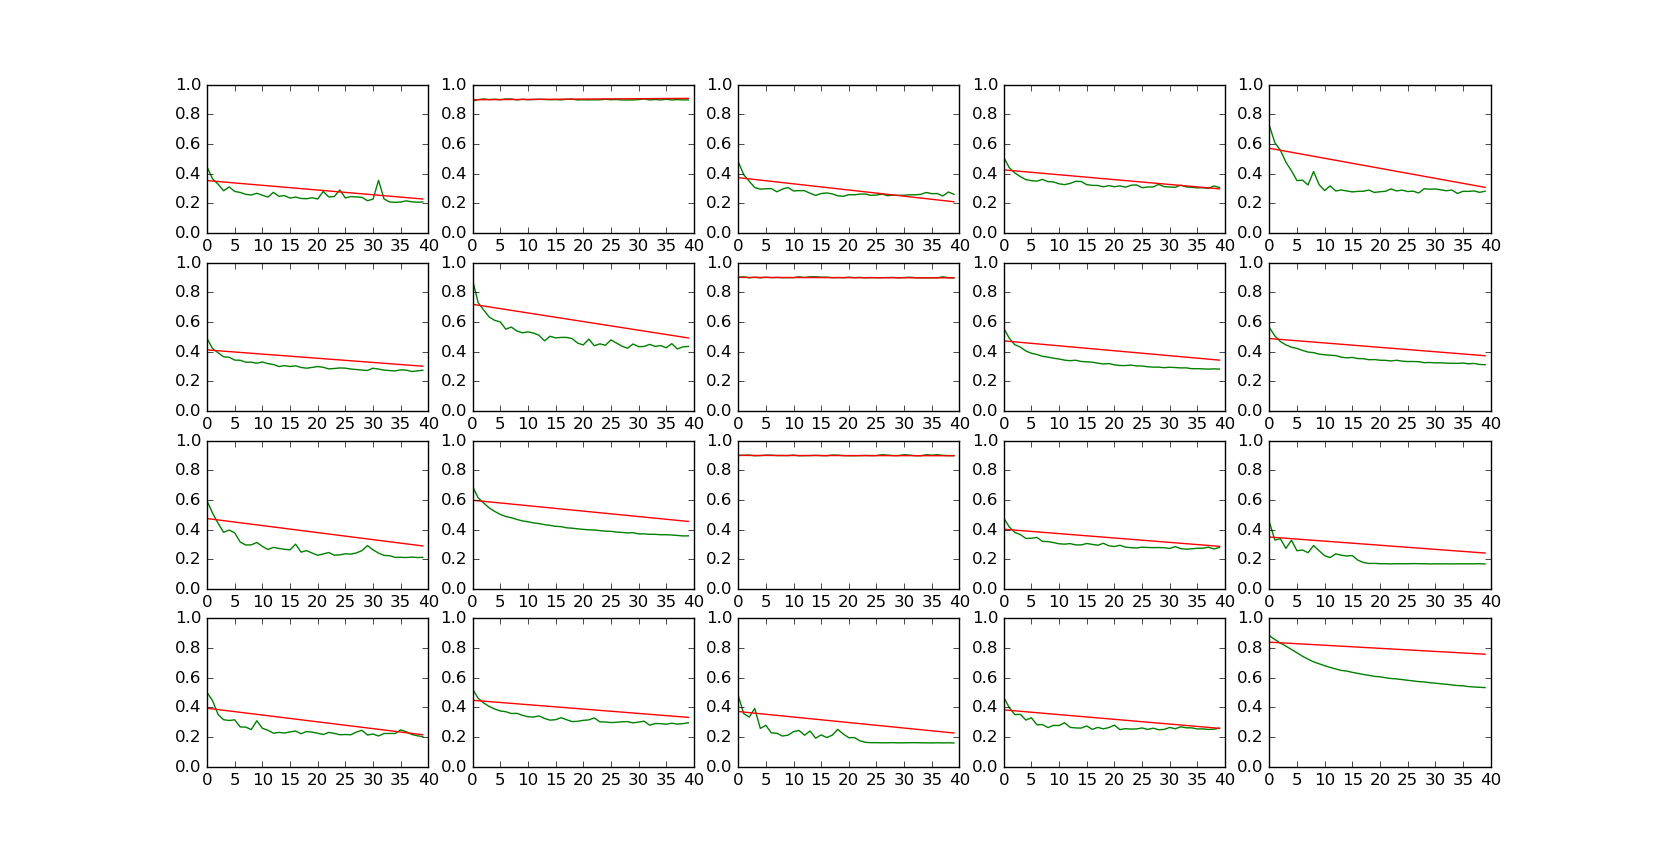
\includegraphics[width=\textwidth]{../../figures/regression_5_lin}

Logarithmic on range (0, 5):

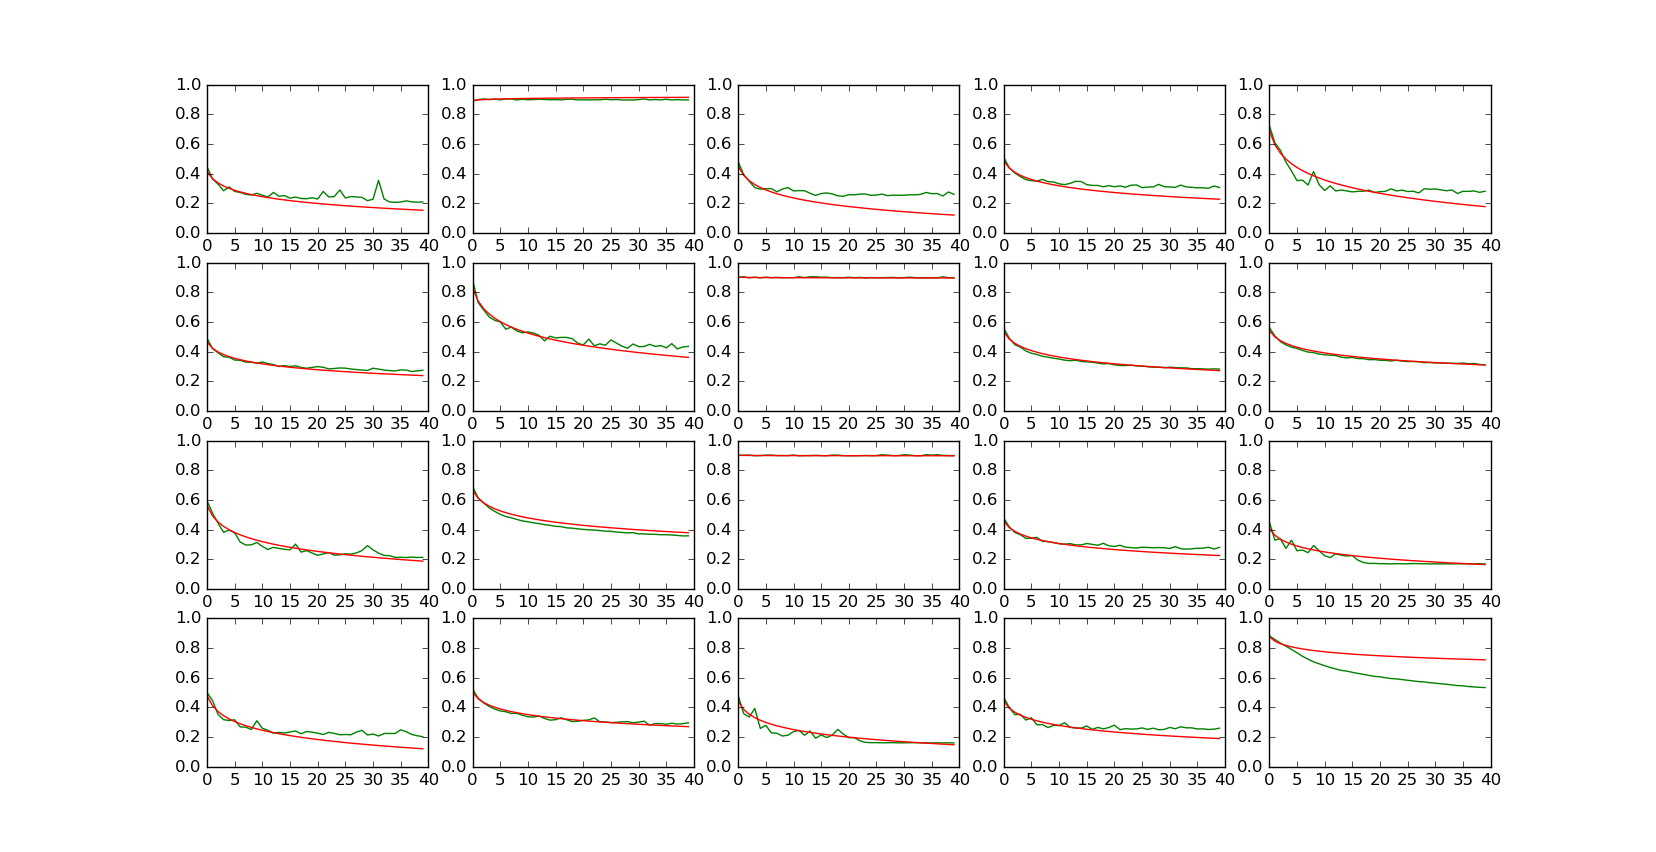
\includegraphics[width=\textwidth]{../../figures/regression_5_log}

Linear on range (0, 10):

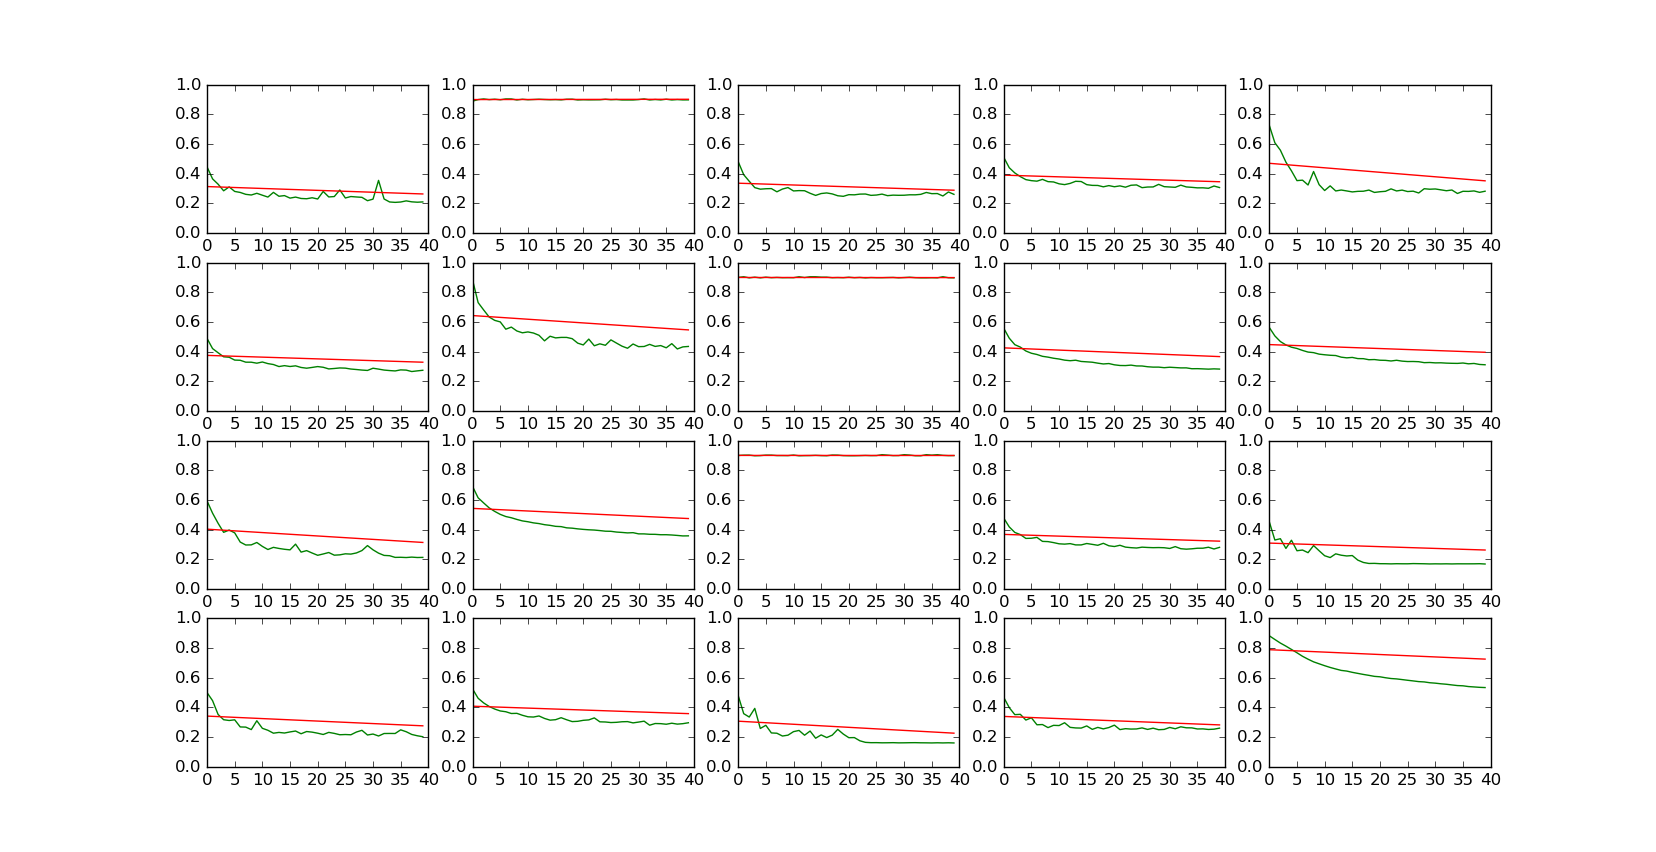
\includegraphics[width=\textwidth]{../../figures/regression_10_lin}

Logarithmic on range (0, 10):

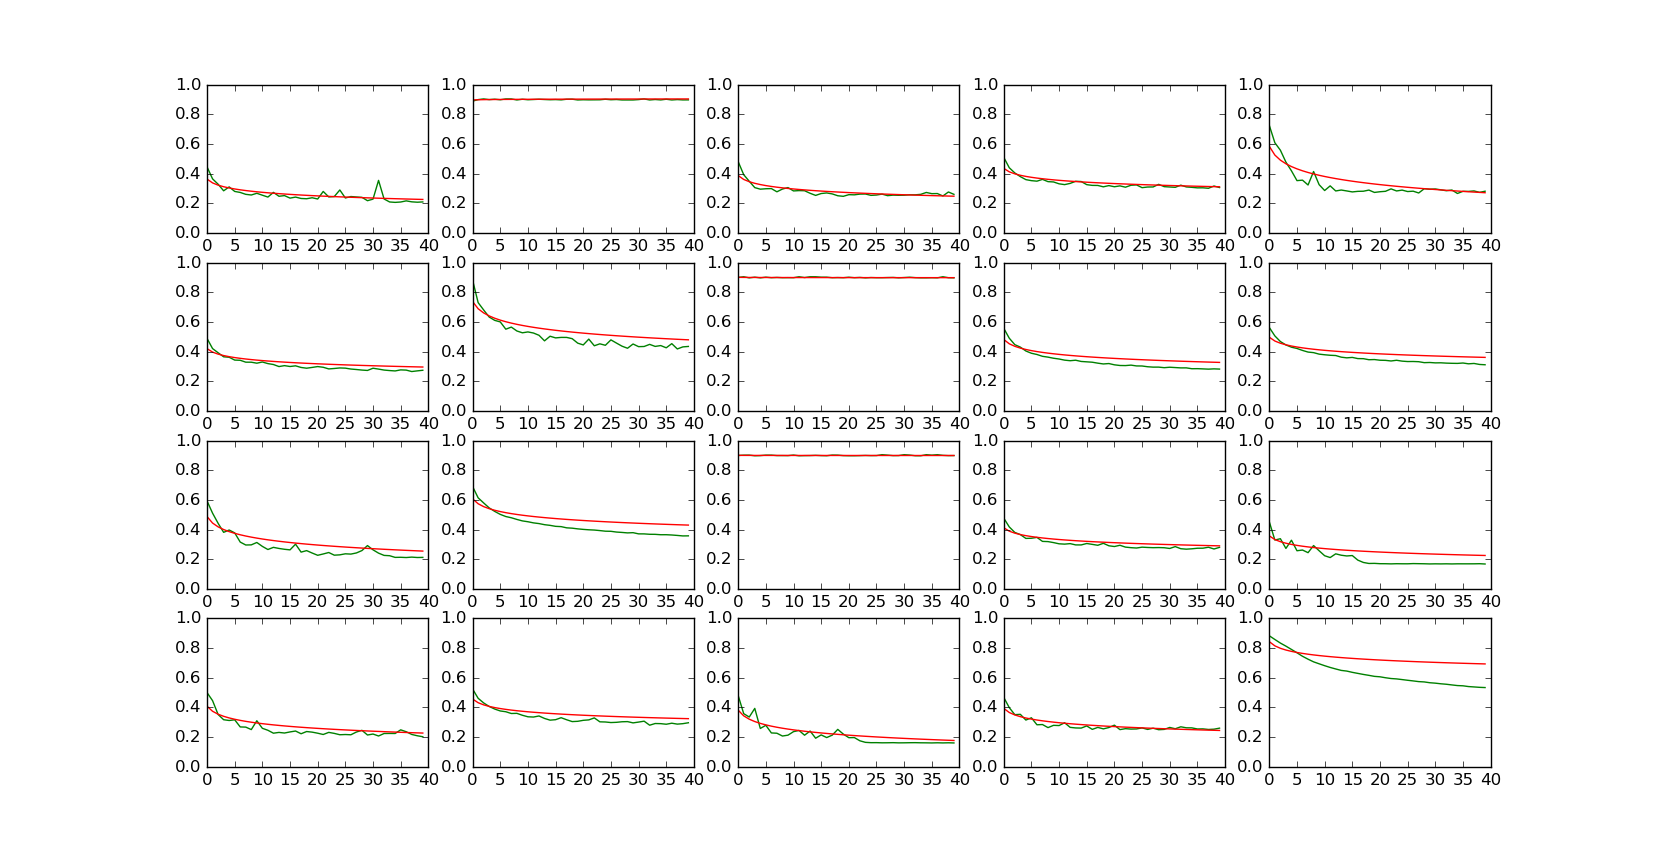
\includegraphics[width=\textwidth]{../../figures/regression_10_log}
Linear on range (10, 20):

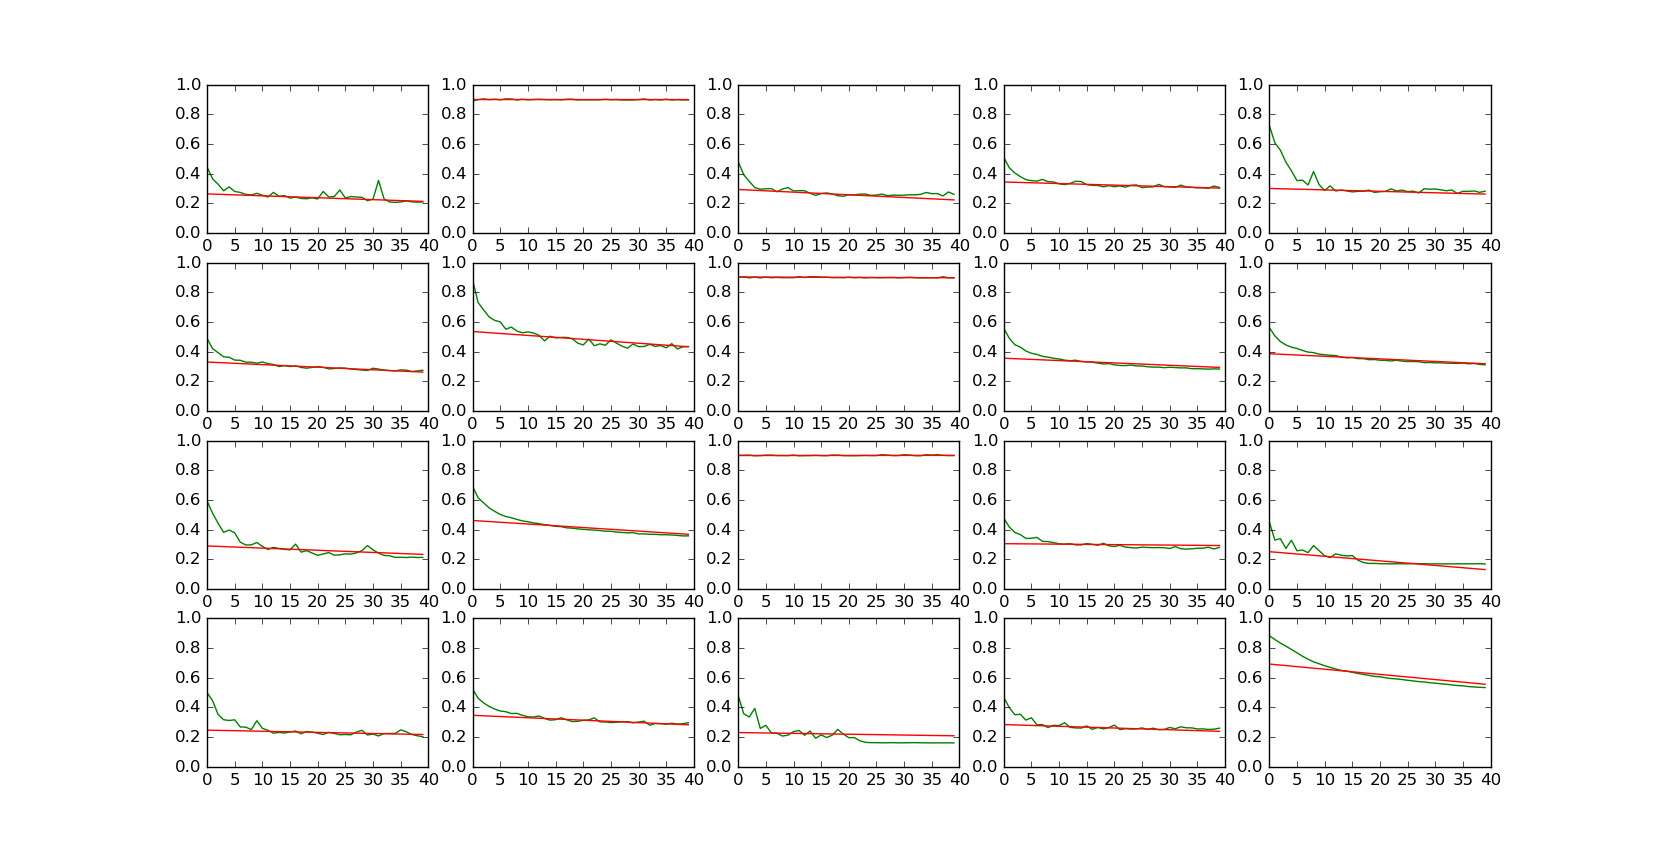
\includegraphics[width=\textwidth]{../../figures/regression_20_lin}

Logarithmic on range (10, 20):

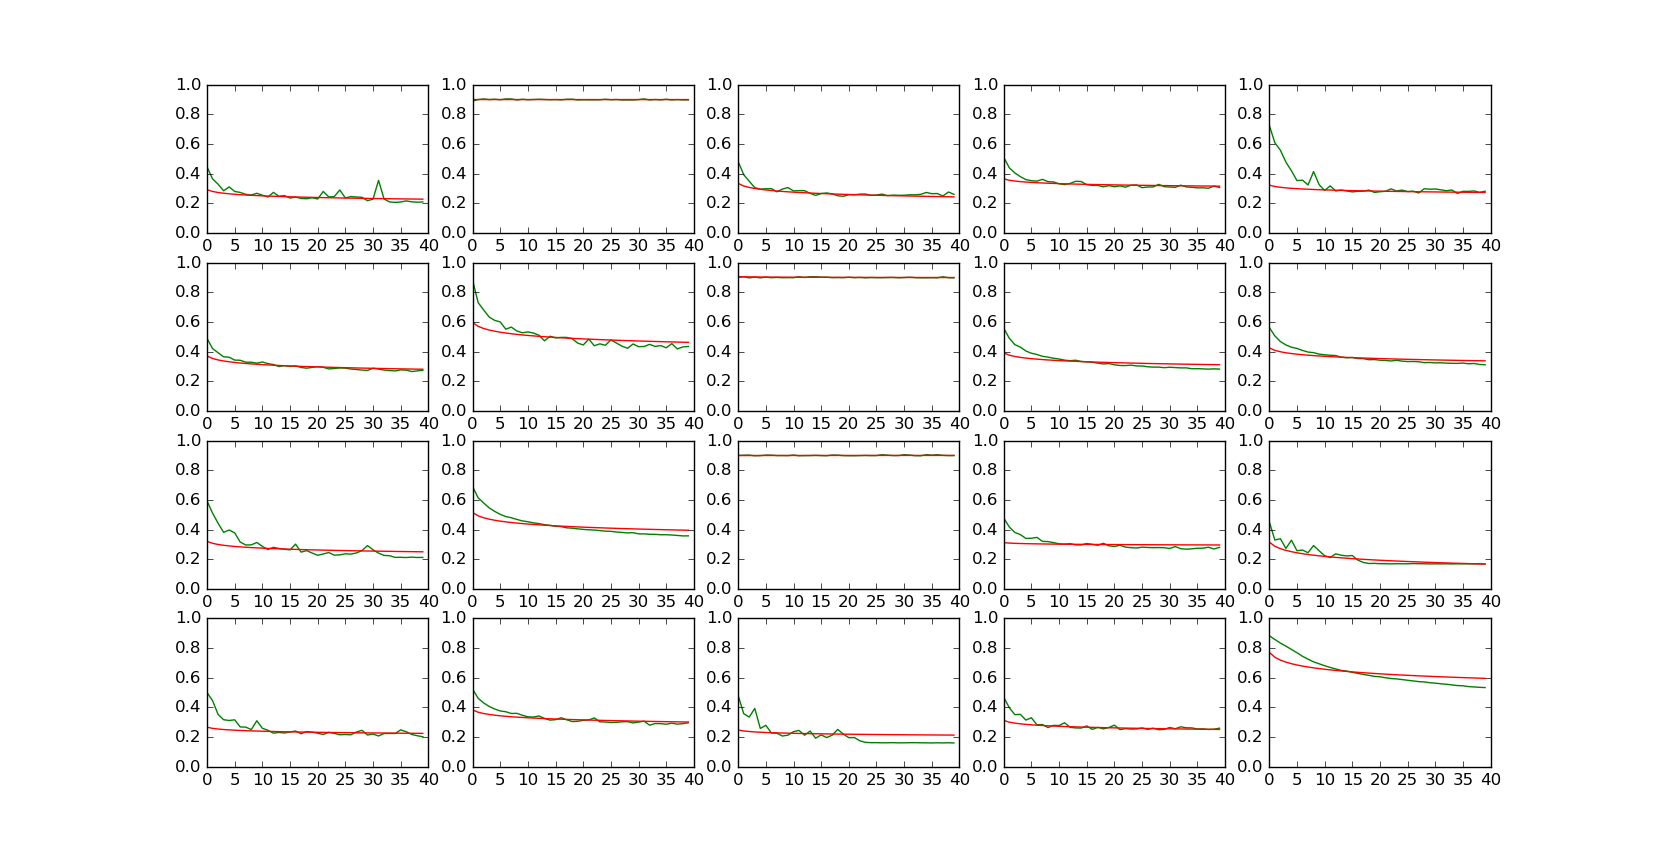
\includegraphics[width=\textwidth]{../../figures/regression_20_log}

\end{document}